% Draft: describes the system as implemented in the colregs-planner
% repository (commit fc6efb4 plus the uncommitted fix that sails the own
% ship's plans as planned near terrain). Numbers in Section 9 are from
% development runs of the milliAmpere scenarios; regenerate before use.
\documentclass[10pt,a4paper]{article}

\usepackage[utf8]{inputenc}
\usepackage[T1]{fontenc}
\usepackage{lmodern}
\usepackage[margin=2.3cm]{geometry}
\usepackage{amsmath,amssymb}
\usepackage{bm}
\usepackage{graphicx}
\usepackage{booktabs}
\usepackage{subcaption}
\usepackage{xcolor}
\usepackage{tikz}
\usetikzlibrary{positioning,arrows.meta,fit}
\usepackage[hidelinks]{hyperref}
\usepackage[capitalise]{cleveref}

\newcommand{\todo}[1]{\textcolor{red}{[TODO: #1]}}
\newcommand{\R}{\mathsf{R}}
\newcommand{\N}{\mathsf{N}}
\DeclareMathOperator{\wrap}{wrap}
\DeclareMathOperator*{\argmin}{arg\,min}

\title{COLREGs-Aware Prediction and Manoeuvre Planning\\[0.3em]}
\date{\today}

\begin{document}
\maketitle

\section{System overview}\label{sec:overview}

Let $\mathcal{V}$ be the set of vessels, $o\in\mathcal{V}$ the own ship.

At each observation time $t_k$ (every $\Delta t$, 0.5\,s in the simulations) the
system runs the following cycle (\cref{fig:overview}): \begin{enumerate} \item
The COLREGs classifier updates the nominal interaction graph $G_{\text{nom}}$
from the observed states (\cref{sec:graph}).  \item Each vessel's responsiveness
filter updates its belief $p_i = p(r_i = \R \mid z_{1:k})$ that vessel $i$
responds to its obligations (\cref{sec:filter}).  \item The joint hypotheses $h
\in \{\R,\N\}^{|\mathcal{V}|}$ are ranked by probability, and the top $K$ are
rolled out over the horizon with the VO policy, each with the graph adjusted for
that hypothesis (\cref{sec:rollout}).  \item Every $T_r$ (5\,s), the own ship
replans: a manoeuvre search scores every action sequence against the top
hypotheses, and the own ship's track along the chosen plan becomes the DP
reference until the next replan (\cref{sec:planner}).  \end{enumerate}

We experiment with how the vessel behaves in constrained waters.

\begin{figure}[t]
\centering
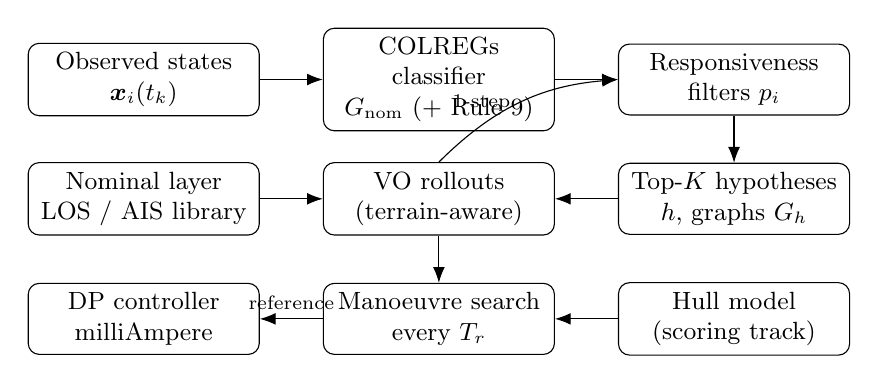
\begin{tikzpicture}[
  node distance=6mm and 8mm,
  box/.style={draw, rounded corners, align=center, minimum height=9mm, text width=27mm, font=\small},
  arr/.style={-{Latex[length=2mm]}}]
  \node[box] (obs) {Observed states\\$\bm{x}_i(t_k)$};
  \node[box, right=of obs] (cls) {COLREGs classifier\\$G_{\text{nom}}$ (+ Rule 9)};
  \node[box, right=of cls] (flt) {Responsiveness\\filters $p_i$};
  \node[box, below=of flt] (hyp) {Top-$K$ hypotheses\\$h$, graphs $G_h$};
  \node[box, left=of hyp] (vo) {VO rollouts\\(terrain-aware)};
  \node[box, left=of vo] (nom) {Nominal layer\\LOS / AIS library};
  \node[box, below=of vo] (plan) {Manoeuvre search\\every $T_r$};
  \node[box, right=of plan] (hull) {Hull model\\(scoring track)};
  \node[box, left=of plan] (dp) {DP controller\\milliAmpere};
  \draw[arr] (obs) -- (cls);
  \draw[arr] (cls) -- (flt);
  \draw[arr] (flt) -- (hyp);
  \draw[arr] (hyp) -- (vo);
  \draw[arr] (nom) -- (vo);
  \draw[arr] (vo) -- (plan);
  \draw[arr] (hull) -- (plan);
  \draw[arr] (plan) -- node[above, font=\scriptsize]{reference} (dp);
  \draw[arr] (vo.north) to[bend left=20] node[left, font=\scriptsize]{1-step} (flt.west);
\end{tikzpicture}
\caption{Processing cycle. One-step VO predictions feed the responsiveness filters; full-horizon rollouts feed the planner, which also uses them to score its own candidate manoeuvres.}
\label{fig:overview}
\end{figure}

\section{Vessel models}\label{sec:models}

\paragraph{Rollout model.} Predicted vessels, and the simulated target vessels, follow a kinematic coordinated-turn model with decoupled heading and speed,
\begin{equation}
  \dot n = U\cos\psi,\qquad \dot e = U\sin\psi,\qquad \dot\psi = r,\qquad r = k_\psi \wrap(\psi_d - \psi),
\end{equation}
driven by a desired velocity $\bm{v}_d$ from the policy, with $\psi_d = \angle\bm{v}_d$ and $U$ set to $\|\bm{v}_d\|$ (optionally through a first-order lag with time constant $\tau_U$, 0 by default). The gain $k_\psi$ (0.1\,s$^{-1}$) gives the gradual turns the responsiveness filter scores against.

\paragraph{milliAmpere-based.} The own ship is simulated with the 3-DOF manoeuvring
model of the milliAmpere autonomous ferry according to Fossen's 3 DOF model.

The ship is actuated by a Dynamic Positioning (DP) system where a reference pose $[x, y, \psi]^\top$ 
is generated from the chosen plan.

\section{Prediction layer}
\subsection{Nominal prediction} \label{sec:nominal}

The nominal layer gives each vessel's preferred velocity without traffic.
It uses basic LOS guidance to follow a straight path.

\subsection{COLREGs interaction graph} \label{sec:graph}

\paragraph{Encounter classification.} 

For every pair $\{a,b\}$ a stateful
classifier assigns an encounter type from
$a$'s perspective: head-on, crossing with $b$ to starboard ($a$ gives way),
crossing with $b$ to port ($a$ stands on), $a$ overtaking $b$, or $b$ overtaking
$a$. The type is looked up in a table of rectangles in the plane of relative
course $\psi_b-\psi_a$ and relative bearing of $b$ from $a$'s course. To be
robust to the instantaneous geometry, both vessels are projected at constant
velocity to their CPA, the table is evaluated at
equally spaced time deltas, and the most frequent label wins, ties going to
the higher-priority label (give-way situations first). A pair gets no new
encounter when its DCPA) exceeds $d_{\text{cpa,max}}$, when it
is farther apart than $d_a$, or when it is not approaching (TCPA $\le 0$).

\paragraph{Hysteresis.} 

An active encounter is kept with a hysteresis score that grows by $w_r$ when the
classification agrees and shrinks by $w_f$ when it does not; it switches only
when the score reaches zero. It is cleared once the vessels are separating, more
than $d_u$ apart and with DCPA above $d_u$, for $n_{\text{clear}}$ consecutive
steps. A confirmed overtaking is held until the overtaking vessel is past the
other's beam.

\paragraph{Roles.}

Each encounter maps to a pair of roles in \{\textsc{give-way},
\textsc{stand-on}, \textsc{head-on}, \textsc{overtaking},
\textsc{avoid-collision}\} (\cref{tab:roles}), forming the graph
$G_{\text{nom}}$ whose edges carry both roles.

\begin{table}[t]
\centering\small
\caption{Encounter types and roles (vessel $a$, vessel $b$), and the role a responsive vessel takes toward a non-responsive one.}
\label{tab:roles}
\begin{tabular}{@{}lll@{\hspace{2em}}ll@{}}
\toprule
Encounter ($a$'s view) & Role $a$ & Role $b$ & Nominal role & Facing a non-responsive vessel\\
\midrule
Head-on & head-on & head-on & head-on & give-way \\
Crossing, $b$ to starboard & give-way & stand-on & stand-on & avoid-collision \\
Crossing, $b$ to port & stand-on & give-way & give-way & give-way \\
$a$ overtaking $b$ & overtaking & stand-on & overtaking & avoid-collision \\
$b$ overtaking $a$ & stand-on & overtaking & avoid-collision & avoid-collision \\
\bottomrule
\end{tabular}
\end{table}

\paragraph{Responsiveness adjustment.} 

Under a hypothesis $h$ a non-responsive vessel holds its nominal track and
ignores all traffic; its role becomes \textsc{stand-on}, and a responsive vessel
facing it takes the role in the right half of \cref{tab:roles}. This gives the
effective graph $G_h$.

\subsection{Responsiveness inference}\label{sec:filter}

Each vessel $i$ has a two-state hidden Markov model for $r_i\in\{\R,\N\}$ (responsive or not), filtered recursively,
\begin{equation}
  p(r_k\mid z_{1:k}) \propto p(z_k \mid r_k)\sum_{r_{k-1}} p(r_k\mid r_{k-1})\,p(r_{k-1}\mid z_{1:k-1}).
\end{equation}

The transition probability $\varepsilon_\R = p(r_k=\N\mid r_{k-1}=\R)$ is
$10^{-5}$ per step, and $\varepsilon_\N = \varepsilon_\R \cdot p_0/(1-p_0)$
makes the prior $p_0 = p(r_0=\R) = 0.99$ the stationary distribution, so the
belief returns to the prior when the evidence is neutral. The likelihood scores
only the observed course $\psi^{\text{obs}}$, with a von Mises density of
concentration $\kappa = 1/\sigma_\psi^2$ (default $\sigma_\psi = 3^\circ$):

\begin{align}
  L_\R &= \sum_{h:\,h_i=\R} w_h\, f_{\text{vM}}\!\left(\psi^{\text{obs}};\,\hat\psi_{i,h},\,\kappa\right), &
  L_\N &= f_{\text{vM}}\!\left(\psi^{\text{obs}};\,\hat\psi_{i}^{\text{nom}},\,\kappa\right).
\end{align}

Here $\hat\psi_{i,h}$ is vessel $i$'s course one step ahead in a one-step VO
rollout of every joint hypothesis in which $i$ is responsive, weighted by the
hypothesis probability $w_h$ (normalised), and $\hat\psi_i^{\text{nom}}$ is its
nominal one-step course. Course is used rather than the full velocity because
Rule 8 favours course changes, so they give the earliest signal. Below 0.5\,m/s
the course is undefined and the likelihood is set to 1, and the belief is held
at the prior for the first 10 steps while the classifier's hysteresis settles.

\subsection{Interaction-aware prediction}\label{sec:rollout}

\subsubsection{Hypotheses}
With the beliefs $p_i$, the probability of a joint hypothesis is
\begin{equation}
  P(h) = \prod_{i} p_i^{[h_i=\R]}\,(1-p_i)^{[h_i=\N]}.
\end{equation}

Vessels whose responsiveness is known, such as the own ship, are fixed. The $K$
most probable hypotheses are each rolled out over the
horizon with their effective graph $G_h$, held fixed or, optionally,
reclassified at every rollout step. A non-responsive vessel follows its nominal
track by LOS and ignores everything.

\subsubsection{COLREGs-aware velocity obstacles}\label{sec:vo} At each rollout step
every responsive vessel selects a velocity with an analytic VO policy.  Speed is
held at the preferred speed $R=\|\bm v_{\text{pref}}\|$, so every response is a
course change on the speed ring $\|\bm v\|=R$, within a course budget
$\pm\theta_b$ ($70^\circ$) of the nominal course.

The obstacles of vessel $i$ are the vessels it has an edge with in $G_h$, or
without a graph, every vessel with TCPA below a threshold. For obstacle $j$ at
distance $d_j$, the cone has its apex at $\bm v_j$, shifted to $\bm v_j +
w_{\text{rvo}}(\bm v_i - \bm v_j)$ for a head-on encounter (a reciprocal
VO with $w_{\text{rvo}}=0.5$: each vessel takes half the
manoeuvre), its axis along the line of sight, and half-angle $\arcsin(r_j/d_j)$.
The radius depends on the role: $D_j = d_{\text{pass}}$ for give-way, head-on,
overtaking and avoid-collision, and $D_j = d_{\text{coll}}$
($0.1\,d_{\text{pass}}$ by default) for stand-on, the last-moment action of Rule
17(b) ($d_{\text{pass}}$ is the desired minimum passing distance). Give-way and head-on also impose a starboard constraint: the vessel may
not converge on the obstacle on its port side. 

The passing distance actually demanded is
\begin{equation}
  r_j = \min(D_j,\ \alpha D_j^*),\qquad D_j^* = d_j \sin\!\big(\min(\phi_{\max},\,90^\circ)\big),
\end{equation}
where $D_j^*$ is the largest passing distance any admissible heading on the ring can achieve against $j$ alone, computed in closed form from the angle $\phi$ between $\bm v - \text{apex}$ and the cone axis. So a vessel keeps the full passing distance when it can and the best reachable one otherwise, and the cone never degenerates when the vessels are already closer than $D_j$. The selected heading minimises
\begin{equation}
  J(\bm v) = |\angle(\bm v,\bm v_{\text{pref}})| + \lambda\,|\angle(\bm v,\bm v_{\text{prev}})|
\end{equation}
over the admissible part of the ring (outside all cones, within the budget, satisfying the starboard constraints), with $\lambda = 0.9$ damping heading switches. The minimum lies at $\bm v_{\text{pref}}$, $\bm v_{\text{prev}}$ or where a constraint boundary meets the ring, so only those candidates are evaluated. If several obstacles together leave no heading, all cones are pulled in by a common velocity shift $\delta$, the smallest that frees a heading (closed form, divided by $\alpha$); this lowers the passing distance to each obstacle by about $\delta\,t_{\text{cpa},j}$, most for encounters farthest ahead. If the starboard constraints exclude each other, the vessel keeps its previous course.

\section{Own-ship manoeuvre planning}\label{sec:planner}

\begin{figure}
  \centering
  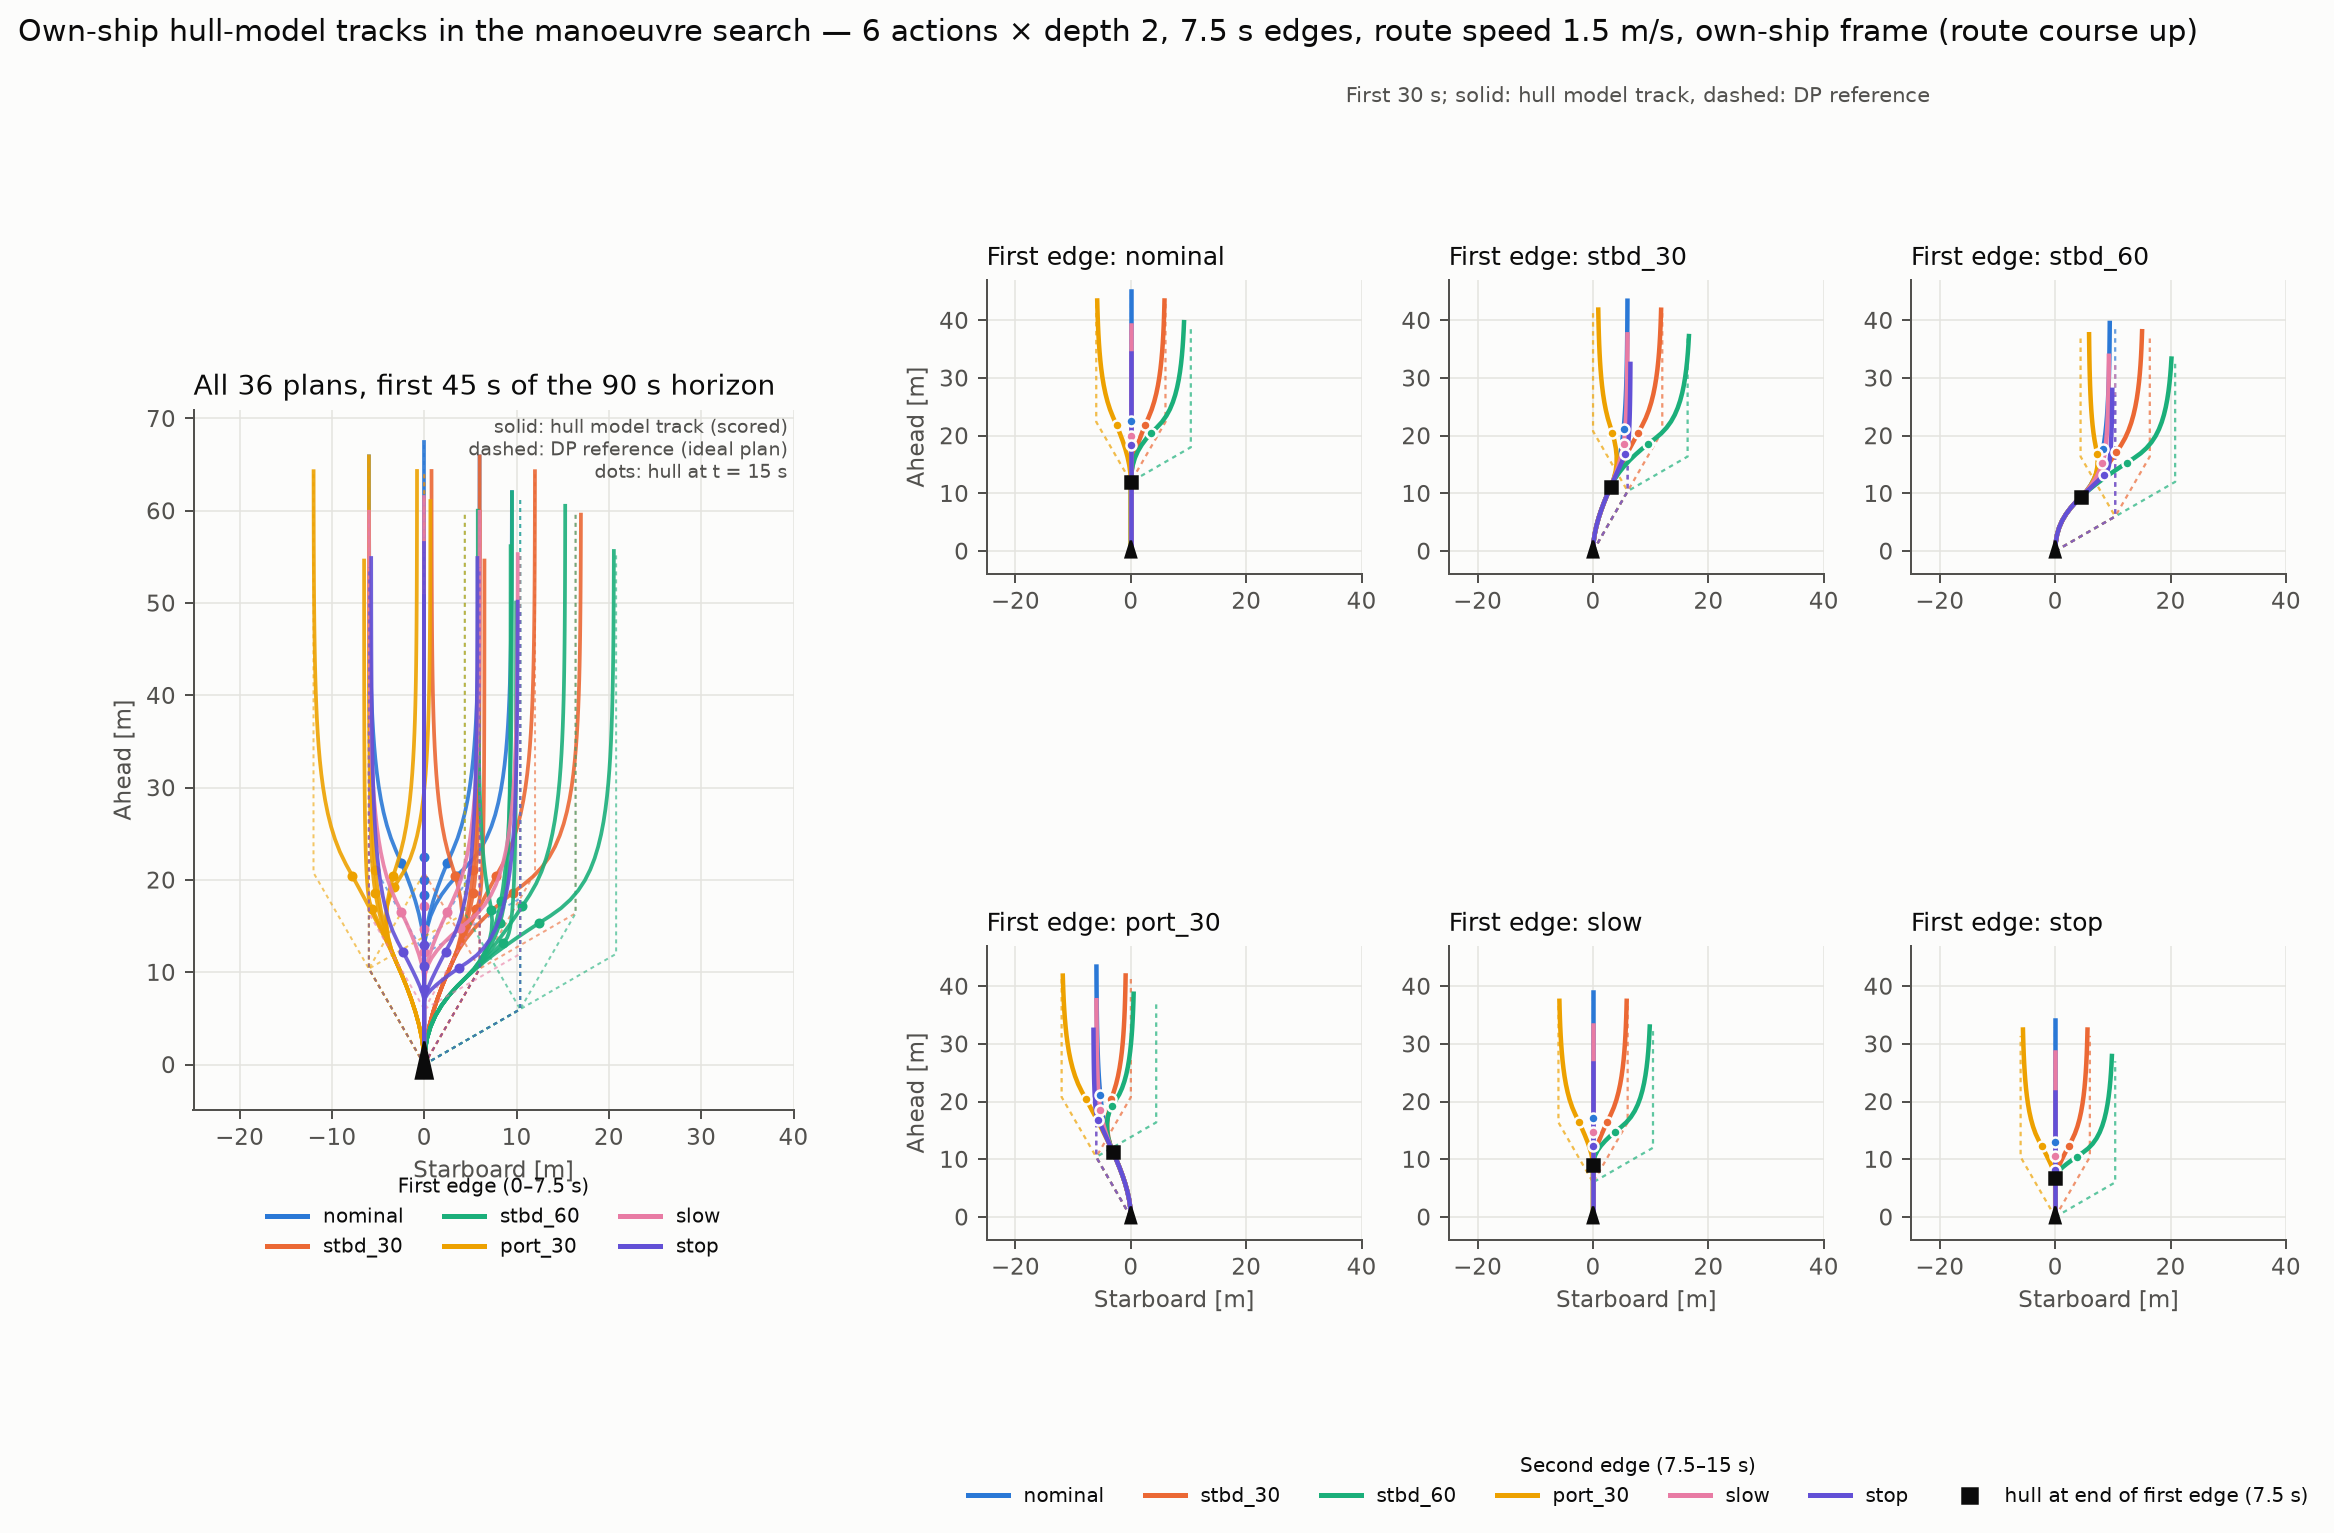
\includegraphics[width=\linewidth]{figures/plan_trajectories_hull.png}
  \caption{The projected trajectory edges generated by the actions when planning forward.}
  \label{fig:trajectories}
\end{figure}

\subsection{Plans}
A plan is a sequence of edges, computed by propagating the vessel at current velocity forward for $T_e = 7.5$\,s, where each edge
is generated from an action 
\[
  \mathcal A = \{\text{nominal},\ \text{stbd}_{30},\ \text{stbd}_{60},\ \text{port}_{30},\ \text{slow},\ \text{stop}\},
\]

a course offset from the route course ($+30^\circ$, $+60^\circ$, $-30^\circ$) or
a speed factor (0.5, 0). 

A DP reference point $\mathbf{\dot{p_r}}$ is generated along these edges relative to the vessel's current position.
In order to capture the vessel dynamics accurately, a closed-loop simulation of a Constant Acceleration (CA) model
is used. This is more accurate than a CV model; stop and slow actions are not assumed to instantly slow or stop
the vehicle. The CA model is described as

\begin{equation}
  \ddot{\bm p} = \operatorname{sat}_{a_{\max}}\!\Big(k_p(\bm p_r - \bm p) + k_d(\dot{\bm p}_r - \dot{\bm p}) - c\,\dot{\bm p}\Big),
\end{equation}

where $k_p$ and $k_d$ are DP tuning constants fitted to the milliAmpere.


See Figure \ref{fig:trajectories} for the tracks that are generated using the CA-model, here the vessel has a reference speed of $v=1.5$ m/s. 
During edge $m$ the planned velocity is the nominal
route velocity rotated by the edge's course offset and scaled by its speed
factor; after the last edge it is the nominal velocity for the rest of the
horizon (90\,s at 1\,s steps), which leaves the ship on a track parallel to the
route. With depth 2 the $|\mathcal A|^2 = 36$ plans are searched exhaustively,
so the result is optimal over the action set.


Each plan is first rolled out alone, without traffic, in fixed-plan mode. This
gives the own-ship reference track. In it the own ship sails the plan as
planned; its VO's terrain check is switched off there. 

The plan is then rolled out with the other vessels using the VO predictor, with
the own ship's track fixed to what was computed using the CA model. The other vessels then
react to each other and the own vessel's interaction behaviour.

When scoring the own ship's plans, we pad the passing distance to $d_s = d_{\text{pass}} + m_{\text{pass}}$
to allow for the remaining prediction error: a plan that only just clears $d_{\text{pass}}$ would
otherwise cost nothing, while the VO vessels keep $d_{\text{pass}}$.

\subsection{Cost} 

\paragraph{Safety margin penalties}

We consider the safety and COLREG penalties over all hypotheses from the rollout. Let $d_j$
be the closest approach to vessel $j$ over the rollout, and $d_s = d_{\text{pass}} + m_{\text{pass}}$
the target passing distance. For a given hypothesis $h$, the safety cost is given as

\begin{align}
  \text{safety}_h &= 
    \sum_j w_{\text{safe}}\max(s_j, b_j)^2 + w_{\text{coll}}[d_j < d_{\text{coll}}],\qquad s_j = \frac{\max(0, d_s - d_j)}{d_s},\\
  b_j &= \frac{\max(0, B - \text{bcr}_j)}{B},\qquad B = f_{\text{bow}}\, d_s,
\end{align}

where $[\cdot]$ is 1 if its condition holds and 0 otherwise, $w_{\text{coll}}$ is the weight penalizing collision
(obviously, this is higher than any other weight), $d_{\text{coll}} = 0.1\,d_{\text{pass}}$, and
$w_\text{safe}$ penalizes closeness when passing or crossing other vessel's heading line (Rule 15: the give-way vessel
avoids crossing ahead). The shortfall $s_j$ is 0 at or beyond $d_s$ and grows linearly to 1 at contact.
$\text{bcr}_j$, the bow crossing range, is how far ahead of vessel $j$ the own ship is when it crosses $j$'s
heading line, at the nearest such crossing in the rollout; without a crossing ahead, $b_j = 0$.
Since the range at a crossing is at least $d_j$, $b_j$ only adds to $s_j$ when $f_{\text{bow}} > 1$; with
$f_{\text{bow}} = 2$, crossing ahead needs twice the room of passing astern. The bow term applies to every
vessel, whatever the own ship's role. Taking the larger of $s_j$ and $b_j$ avoids counting one encounter twice,
and squaring it keeps small shortfalls cheap and large ones expensive.


\paragraph{COLREG-specific penalties}
The COLREGs term
$\text{colregs}_h$ sums indicator penalties:

\begin{itemize}
  \item $w_{\text{port}}$ for any port offset while give-way or head-on to a vessel, or for any edge that turns toward a vessel being overtaken;
  \item $w_{\text{give}}$ if the first edge does not alter to starboard while head-on to a vessel it is in conflict with (Rule 14), keeps course and speed while give-way to one (Rule 16), or does not alter away from a vessel it is overtaking and in conflict with (Rules 13, 16);
  \item $w_{\text{stand}}$ for manoeuvring on the first edge while stand-on to a vessel responsive under $h$, unless bound to keep clear of another vessel (Rule 17(a)(i)).
\end{itemize}
A vessel is in conflict while resuming the route course from the current position would pass it inside its role's passing distance; once the manoeuvre has opened that distance, holding course is no longer penalised. Roles only count toward vessels still approaching. For a vessel being overtaken, the TCPA is taken on the route course, the encounter only costs a collision until it is within the predictor's TCPA threshold, and from then on $d_j$ also includes the straight-line CPA after the horizon, since overtaking closes slowly and the pass often lies beyond it.

\paragraph{Grounding} (Work in progress)

Letting $g$ be the distance to the closest hazard during the planned trajectory, and $d_{\text{shore}}$ the safety margin from the vessel's center point, then let

\begin{equation}
  c_{\text{shore}} = w_{\text{ground}}\Big(\frac{\max(0, d_{\text{shore}} - g)}{d_{\text{shore}}}\Big)^2 + w_{\text{aground}}[g<0]
\end{equation}

\paragraph{Time and effort}

We want to minimize effort by penalizing unnecessary deviation and course changes. Letting $m = 1, \dots, D$
index the edges of the candidate plan ($D = 2$ is the search depth), $\delta_m$ be edge $m$'s course offset
from the route course, and $[\text{slowed or stop}]$ indicate a speed factor below 1, each edge is charged
$|\delta_m|/60^\circ + [\text{slowed or stop}]$ in proportion to the time $T_e$ it is held.

Furthermore, we want to minimize the total time of the avoidance manoeuvre.
Defining the time lost as

\begin{equation}
  T_{\text{lost}} = \max{\left(0, T_H - \frac{\text{progress}}{U_{\text{ref}}}\right)}
\end{equation}

where $T_H = H\,\Delta t_{\text{planner}}$ (90\,s) is the planning horizon, \textit{progress}
is the distance the own ship covers along the route direction over the horizon, measured from its current
position along the scored track (sideways motion does not count), and $U_{\text{ref}}$ is the own ship's
reference speed. $T_{\text{lost}}$ is thus how much less than $T_H$ the same progress would take at the
reference speed. Ignoring hull lag, one edge of $\text{stbd}_{30}$ loses $T_e(1-\cos 30^\circ) \approx 1$\,s,
one of $\text{stbd}_{60}$ or slow 3.75\,s, and one of stop 7.5\,s. A plan cannot earn credit for being ahead
of the reference.

Finally, the effort is divided by $T_{\text{eff}}$ so that it does not depend on the edge length: an edge
counts in full when held for $T_{\text{eff}}$, and twice as many edges of half the length cost the same.
The time lost is divided by $T_{\text{ref}}$, which sets its scale: losing $T_{\text{ref}}$ costs $w_{\text{time}}$.


Deviation from the route is penalized by the mean squared cross-track error over the plan rollout,
normalized by $d_{\text{pass}}$:

\begin{equation}
c_{\text{dev}} = \frac{w_{\text{dev}}}{H+1} \sum_{k=0}^{H} \left(\frac{y(k\,\Delta t_{\text{planner}})}{d_{\text{pass}}}\right)^2
\end{equation}

where $y(t)$ is the own ship's signed perpendicular distance from the route line, positive to starboard.
A plan ends on a track parallel to the route, so an offset built up on its edges is held for the rest of
the horizon, and only a $\text{port}_{30}$ edge brings the ship back. This term is what makes the search
return: it does so once the deviation saved outweighs the effort and time of the return edge. It is
averaged over the horizon rather than taken at its end, since an end-only term would tie ``return now''
with ``return on the next edge'', and replanning would then postpone the return indefinitely.
Normalizing by $d_{\text{pass}}$ makes the term dimensionless, so one $w_{\text{dev}}$ serves every
scenario scale, and keeps its balance with the safety term, which is normalized by $d_s$, the same
across scenarios. A give-way manoeuvre must open roughly $d_{\text{pass}}$ sideways; held for the whole
horizon, that offset costs $w_{\text{dev}}$, far less than a shortfall in passing distance, so the term
never holds back a manoeuvre.

This gives the  total time and effort cost

\begin{equation}
  c_{te} = 
   w_{\text{eff}}\sum_m\Big(\tfrac{|\delta_m|}{60^\circ} + [\text{slowed or stop}]\Big)\frac{T_e}{T_{\text{eff}}}
       + w_{\text{time}}\frac{T_{\text{lost}}}{T_{\text{ref}}} + c_{\text{dev}}
\end{equation}


\paragraph{Total cost}

The total cost is
\begin{align}
  c = {}& c_{te} + c_{\text{shore}} + \sum_h w_h(\text{safety}_h + \text{colregs}_h) +
   w_{\text{risk}}\max_{h:\,w_h \ge w_{\min}} \text{safety}_h
  \label{eq:cost}
\end{align}

We weigh each of the hypothesis-dependent COLREG and safety costs by the renormalised weight $w_h$ of the
hypothesis, i.e.\ the predictor's probability that it occurs. Furthermore, we add the worst safety cost
over the hypotheses with weight at least $w_{\min}$, so that a plausible hypothesis in which the plan ends
in a close pass or collision is penalized beyond its probability. The floor keeps unlikely hypotheses out:
over all of them, a 1\,\% hypothesis that the give-way vessel never acts would make a stand-on own ship
manoeuvre from the first step.

Safety enters both as expectation and as worst case, but the COLREGs term only as expectation. A rule
penalty is not physical harm, so there is no tail risk to guard against, and it should count in proportion
to how likely it is to apply. Most COLREGs penalties depend only on the plan and on conflicts judged on
the route course, so they are the same under every hypothesis, and a worst-case copy would merely double
their weights against safety. The stand-on penalty, which does depend on $h$, should fade as the filter
comes to doubt the give-way vessel, so that the own ship may act (Rule 17(a)(ii)); in the worst case it
would stay in full until that doubt passed $1 - w_{\min}$. Keeping the worst-case term to safety also
keeps the hysteresis' ``less safe'' test (\cref{sec:hysteresis}) free of rule penalties.

All default weights are in \cref{tab:params}.

\subsection{Plan hysteresis}\label{sec:hysteresis}

Replanning every 5\,s with 7.5\,s edges could
switch plans on noise. The plan in force, adopted at $t_0$, is continued edge by
edge: at time $t$ its continuation is its actions from edge $\lfloor
(t-t_0)/T_e\rfloor$ on, padded with nominal, each at full length. That
continuation is one of the 36 plans and is scored anyway; it is kept unless the
cheapest plan beats it by more than $\max(0.1,\ 0.15\,c_{\text{kept}})$, or it
is less safe (its safety, risk and grounding cost exceed the cheapest plan's).




\appendix
\section{Parameters}\label{app:params}

\begin{table}[h]
\centering\small
\caption{Default parameters.}
\label{tab:params}
\begin{tabular}{@{}llr@{}}
\toprule
Component & Parameter & Default \\
\midrule
Classifier & $d_{\text{cpa,max}}$, $d_a$, $d_u$ & 1500\,m, 10\,km, 150\,m (scaled by 0.3 for milliAmpere) \\
           & $n_t$, $w_r$, $w_f$, $n_{\text{clear}}$ & 11, 1, 0.01, 5 \\
Filter     & $p_0$, $\varepsilon_\R$, $\sigma_\psi$, warm-up & 0.99, $10^{-5}$, $3^\circ$, 10 steps \\
VO         & $\theta_b$, $\lambda$, $\alpha$, $w_{\text{rvo}}$ & $70^\circ$, 0.9, 1, 0.5 \\
           & $d_{\text{coll}}$, $k_\psi$ & $0.1\,d_{\text{pass}}$, 0.1\,s$^{-1}$ \\
           & $T_{\text{look}}$, $c_t$ & 30\,s, 5\,m \\
Search     & depth, $T_e$, step, horizon, $K$ & 2, 7.5\,s, 1\,s, 90\,s, 2 \\
           & $T_r$ & 5\,s \\
Cost       & $w_{\text{safe}}$, $w_{\text{coll}}$, $f_{\text{bow}}$ & 100, 1000, 2 \\
           & $w_{\text{port}}$, $w_{\text{give}}$, $w_{\text{stand}}$ & 20, 5, 10 \\
           & $w_{\text{dev}}$, $w_{\text{eff}}$, $w_{\text{time}}$, $T_{\text{eff}}$, $T_{\text{ref}}$ & 2, 1, 1, 15\,s, 15\,s \\
           & $w_{\text{risk}}$, $w_{\min}$, $m_{\text{pass}}$ & 1, 0.1, 6\,m \\
           & $w_{\text{ground}}$, $w_{\text{aground}}$, $d_{\text{shore}}$ & 100, 1000, 8\,m \\
Hysteresis & absolute, relative margin, safety tolerance & 0.1, 0.15, 0 \\
Hull model & $k_p$, $k_d$, $c$, $a_{\max}$, step & 0, 0.20\,s$^{-1}$, 0, 0.17\,m/s$^2$, 0.1\,s \\
\bottomrule
\end{tabular}
\end{table}


\end{document}
